%!TEX root = 0_architecture_rapport.tex

% subsection title
\subsection{Question 1}
\label{subsec:411}

\paragraph{}Below is the database structure of the differents tables. In total, there are 7 tables. The principal key for tables in figure \ref{fig:411-1}, \ref{fig:411-2}, \ref{fig:411-3} and \ref{fig:411-4} is \texttt{playerid}. For others tables, figure~\ref{fig:411-5}, \ref{fig:411-6} and \ref{fig:411-7}, the principal key is \texttt{teamid}.

\begin{figure}[h!]
	\begin{center}
		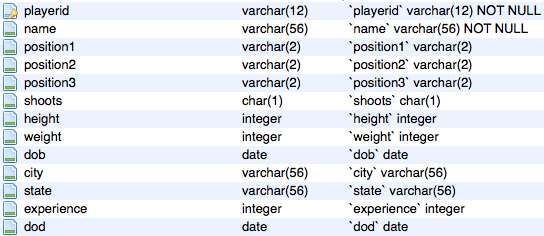
\includegraphics[width=0.7\textwidth]{./images/profile}
		\caption{Profile table schema. \textit{Source: SQLite Browser}}
		\label{fig:411-1}
	\end{center}
\end{figure}

\begin{figure}[h!]
	\begin{center}
		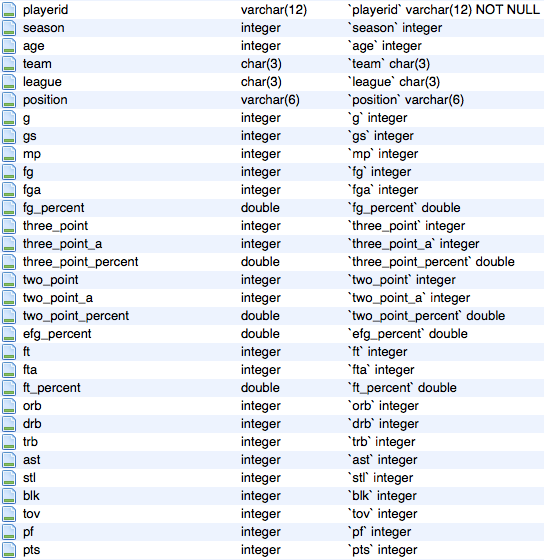
\includegraphics[width=0.7\textwidth]{./images/player_total}
		\caption{Player's Totals table schema \textit{Source: SQLite Browser}}
		\label{fig:411-2}
	\end{center}
\end{figure}

\begin{figure}[h!]
	\begin{center}
		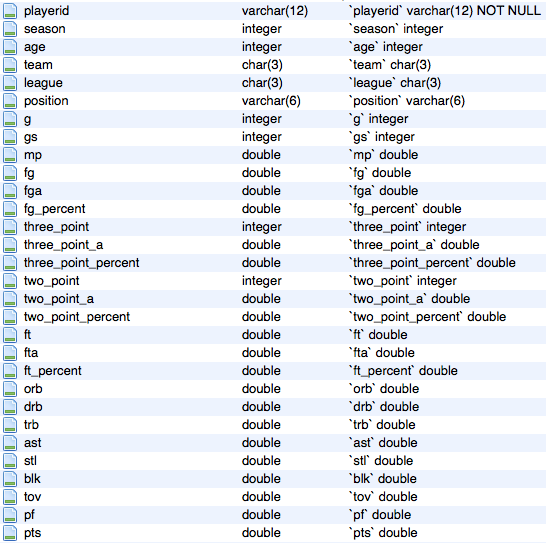
\includegraphics[width=0.7\textwidth]{./images/player_per_game}
		\caption{Player's Per Game table schema \textit{Source: SQLite Browser}}
		\label{fig:411-3}
	\end{center}
\end{figure}

\begin{figure}[h!]
	\begin{center}
		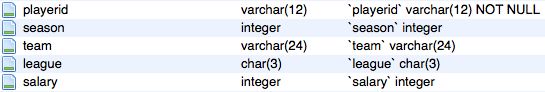
\includegraphics[width=0.7\textwidth]{./images/salary}
		\caption{Salary table schema \textit{Source: SQLite Browser}}
		\label{fig:411-4}
	\end{center}
\end{figure}

\begin{figure}[h!]
	\begin{center}
		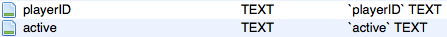
\includegraphics[width=0.7\textwidth]{./images/activeplayers}
		\caption{Active Players table schema \textit{Source: SQLite Browser}}
		\label{fig:411-5}
	\end{center}
\end{figure}

\begin{figure}[h!]
	\begin{center}
		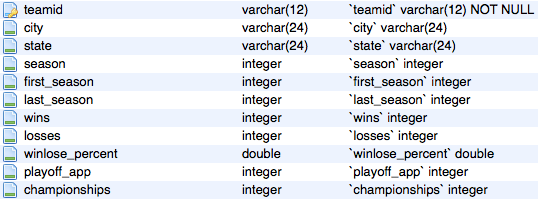
\includegraphics[width=0.7\textwidth]{./images/teaminfo}
		\caption{Team Information table schema \textit{Source: SQLite Browser}}
		\label{fig:411-6}
	\end{center}
\end{figure}

\begin{figure}[h!]
	\begin{center}
		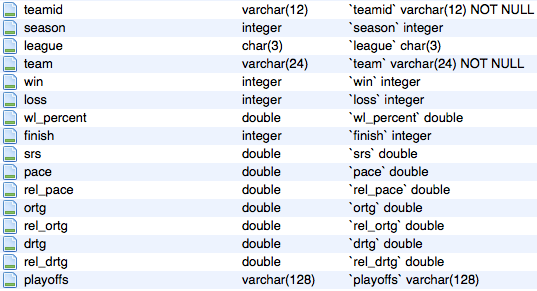
\includegraphics[width=0.7\textwidth]{./images/teamstats}
		\caption{Team Statistics table schema \textit{Source: SQLite Browser}}
		\label{fig:411-7}
	\end{center}
\end{figure}